\subsection{UC1 - Autenticazione}
\begin{itemize}
    \item \textbf{Identificativo}: UC1
    \item \textbf{Nome}: Gestione autenticazione
    \item \textbf{Descrizione grafica}:
\end{itemize}

\begin{figure}[h]
    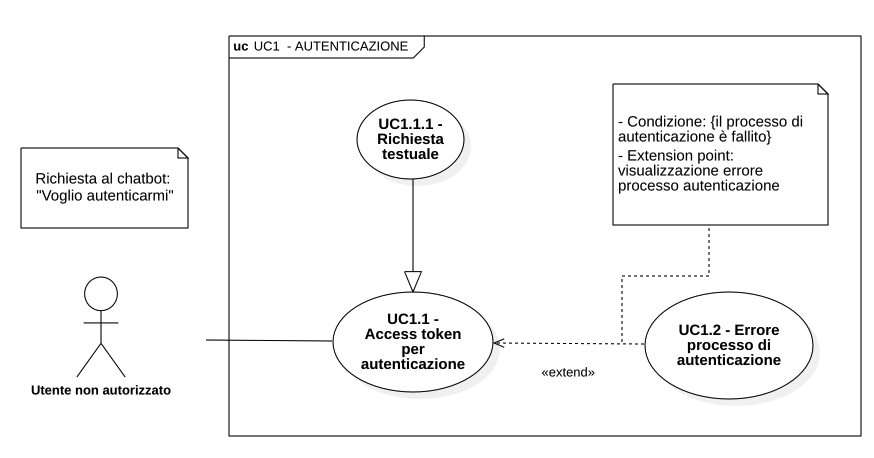
\includegraphics[scale=0.50]{images/UC1.png} 
    \caption{Descrizione grafica caso d'uso UC1}
\end{figure}

 \begin{itemize}
    \item \textbf{Attori}
 \begin{itemize} 
    \item \textit{Primari}: utente non autorizzato
    \item \textit{Secondari}: non presenti
 \end{itemize}
 \item \textbf{Precondizione}: l'utente vuole utilizzare i servizi messi a disposizione dal chatbot e dispone di un access token\textsubscript{G}.
 \item \textbf{Postcondizione}: l'utente si autentica al sistema e può utilizzare il servizio.
 \item \textbf{Scenario principale}: l'utente vuole effettuare il login al sistema, ha a disposizione un access token\textsubscript{G} che fornirà al chatbot per autenticarsi.
 \item \textbf{Scenario secondario:} se l'utente prova ad autenticarsi con un token\textsubscript{G} di accesso non valido viene visualizzato un messaggio di errore. (\textbf{UC1.2})
\end{itemize}
\newpage

\subsubsection{UC1.1 - Token di accesso autenticazione}
\begin{itemize}
    \item \textbf{Identificativo}: UC1.1
    \item \textbf{Nome}: token\textsubscript{G} di accesso autenticazione
    \item \textbf{Descrizione grafica}: (approfondita in UC1)
    \item \textbf{Attori}
 \begin{itemize} 
    \item \textit{Primari}: utente non autorizzato
    \item \textit{Secondari}: non presenti
 \end{itemize}
 \item \textbf{Precondizione}: l'utente ha a disposizione un token\textsubscript{G} di accesso.
 \item \textbf{Postcondizione}: l'utente fornisce il token\textsubscript{G} al chatbot.
 \item \textbf{Scenario principale}: l'utente fornisce il token\textsubscript{G} al chatbot in maniera testuale (UC1.1.1). Se il token\textsubscript{G} fornito è valido allora l'utente avrà effettuato il login correttamente e potrà usufruire dei servizi messi a disposizione. 
 \item \textbf{Scenario secondario}: se il token\textsubscript{G} non risultasse essere valido, verrà mostrato un messaggio di errore ad esso relativo (\textbf{UC1.2})
\end{itemize}

\paragraph{UC1.1.1 - Richiesta Testuale}
\begin{itemize}
   \item \textbf{Identificativo}: UC1.1.1
   \item \textbf{Nome}: Richiesta testuale
   \item \textbf{Descrizione grafica}: (approfondita in UC1)
   \item \textbf{Attori}:
   \begin{itemize} 
       \item \textit{Primari}: utente autorizzato
       \item \textit{Secondari}: non presenti
   \end{itemize}
       \item \textbf{Precondizione}: l'utente dispone del proprio accesso token\textsubscript{G}
       \item \textbf{Postcondizione}: l'utente ha comunicato al chatbot il proprio access token, tramite input testuale. 
    \item \textbf{Scenario principale}: 
       \begin{itemize}
           \item L'utente fornisce un input testuale al chatbot contenente il proprio accesso token\textsubscript{G} 
       \end{itemize}
\end{itemize}

\subsubsection{UC1.2 - Token non valido}
\begin{itemize}
    \item \textbf{Identificativo}: UC1.2
    \item \textbf{Nome}: token\textsubscript{G} non valido
    \item \textbf{Descrizione grafica}: (approfondita in UC1)
    \item \textbf{Attori}
 \begin{itemize} 
    \item \textit{Primari}: utente non autorizzato 
    \item \textit{Secondari}: non presenti
 \end{itemize}
 \item \textbf{Precondizione}: l'utente ha a disposizione un token\textsubscript{G} non valido.
 \item \textbf{Postcondizione}: chatbot nega l'accesso ai servizi, viene comunicato l'errore all'utente e riproposto il sistema di login.
 \item \textbf{Scenario principale}: il token\textsubscript{G} inserito dall'utente risulta essere non valido per l'accesso, viene mostrato un messaggio di errore e il chatbot propone all'utente di rieffettuare la procedura di login.
\end{itemize}
\newpage